%%%%%%%%%%%%%%%%%%%%%%%%%%%%%%%%%%%%%%%%%%%%%%%%%%%%%%%%%%%%%%%%%%%%%%%%
% Plantilla TFG/TFM
% Escuela Politécnica Superior de la Universidad de Alicante
% Realizado por: Jose Manuel Requena Plens
% Contacto: info@jmrplens.com / Telegram:@jmrplens
%%%%%%%%%%%%%%%%%%%%%%%%%%%%%%%%%%%%%%%%%%%%%%%%%%%%%%%%%%%%%%%%%%%%%%%%

\chapter{Resultados (Con ejemplos de gráficos)}
\label{resultados}

\section{Diagramas}
Gracias al paquete \textit{Tikz} se pueden incluir multitud de medios gráficos, diagramas, capas sobre imágenes, etc.
Existen múltiples formas de realizarlo, para ello es recomendable consultar la guía de iniciación disponible aquí: \url{http://cremeronline.com/LaTeX/minimaltikz.pdf} y también el manual completo disponible aquí: \url{http://osl.ugr.es/CTAN/graphics/pgf/base/doc/pgfmanual.pdf}.
\\
\par A continuación se muestran algunos ejemplos. Revisa el archivo .tex para ver cómo se utilizan.
\\
\par Imagen a la que se le ha añadido cuadros y texto desde latex:
\begin{figure}[ht]
\centering	
\resizebox{0.6\textwidth}{!}{%
\begin{tikzpicture}[x=39, y=47]%X,Y -> Corrección de coordenadas, según tamaño y posición de la imagen
    \node[anchor=south west,inner sep=0] (image) at (0,0) {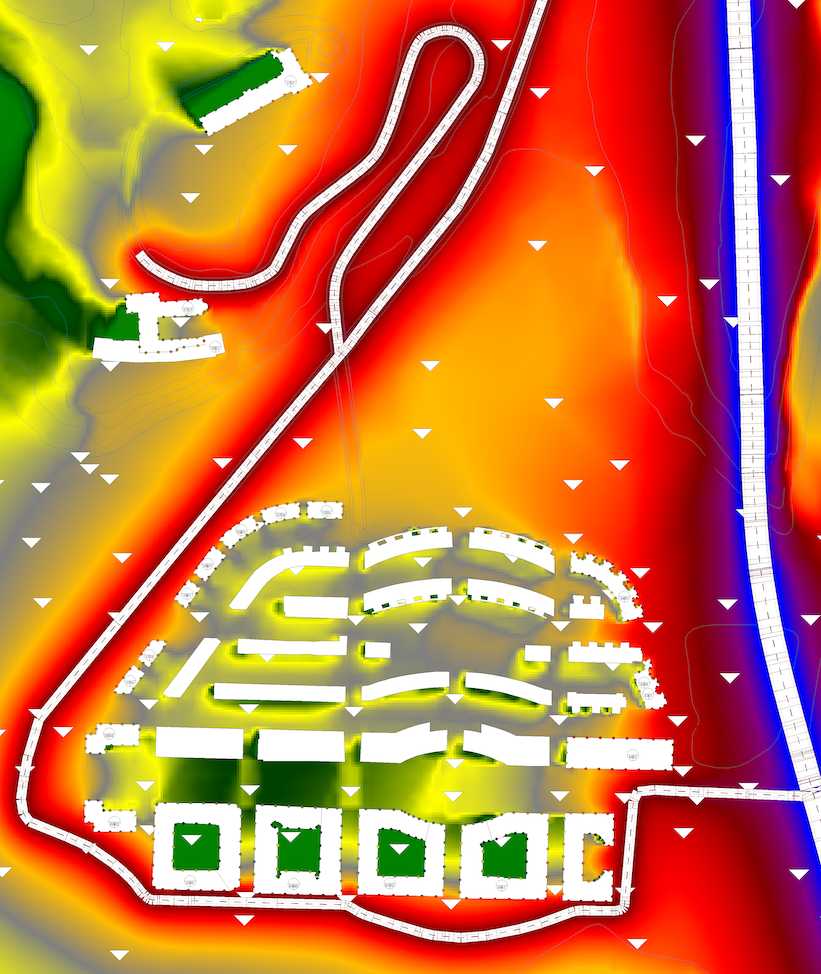
\includegraphics[width=0.9\textwidth]{archivos/mapadia}};
    % Imprimir coordenadas
    \begin{scope}[x={(image.south east)},y={(image.north west)}]
        \draw[help lines,xstep=.1,ystep=.1] (0,0) grid (1,1);
        \foreach \x in {0,1,...,9} { \node [anchor=north] at (\x/10,0) {\x}; }
        \foreach \y in {0,1,...,9} { \node [anchor=east] at (0,\y/10) {\y}; }
    \end{scope}
    % Residencias 1
    \draw[Caja1] (6.8,2) rectangle (8.3,4.5);
    \node[Texto2] at (6.8,2) {\textbf{Residencias 1}};
    % Residencias 2
    \draw[Caja1] (1,0.6) rectangle (7.6,1.8);
    \node[Texto2] at (1,0.6) {\textbf{Residencias 2}};
    % Residencias 3
    \draw[Caja1,rotate around={-45:(2.6,3.6)}] (2.6,3.6) ellipse (1cm and 3.1cm);
    \node[Texto2] at (1.2,2.1) {\textbf{Residencias 3}};
    % Hospital
    \draw[Caja1] (1,6) rectangle (3,7);
    \node[Texto2] at (1,6) {\textbf{Hospital}};
    % Colegio
    \draw[Caja1] (2.3,8.5) rectangle (3.9,9.5);
    \node[Texto2] at (2.3,8.5) {\textbf{Colegio}};
    % Numeros de edificios
    \node[Texto3,font=\tiny] at (7.5,4) {\textbf{1}};
    \node[Texto3,font=\tiny] at (7.9,2.9) {\textbf{2}};
    \node[Texto3,font=\tiny] at (7.7,2.3) {\textbf{3}};
    \node[Texto3,font=\tiny] at (7.2,1.2) {\textbf{4}};
    \node[Texto3,font=\tiny] at (6.2,1.2) {\textbf{5}};
    \node[Texto3,font=\tiny] at (4.9,1.2) {\textbf{6}};
    \node[Texto3,font=\tiny] at (3.6,1.2) {\textbf{7}};
    \node[Texto3,font=\tiny] at (2.4,1.2) {\textbf{8}};
    \node[Texto3,font=\tiny] at (1.5,1.7) {\textbf{9}};
    \node[Texto3,font=\tiny] at (1.5,2.5) {\textbf{10}};
    \node[Texto3,font=\tiny] at (1.5,3) {\textbf{11}};
    \node[Texto3,font=\tiny] at (1.8,3.4) {\textbf{12}};
    \node[Texto3,font=\tiny] at (2.2,3.8) {\textbf{13}};
    \node[Texto3,font=\tiny] at (2.5,4.2) {\textbf{14}};
    \node[Texto3,font=\tiny] at (3,4.5) {\textbf{15}};
    \node[Texto3,font=\tiny] at (3.4,4.8) {\textbf{16}};
    \node[Texto3,font=\tiny] at (4,4.8) {\textbf{17}};
    % Nombres de carreteras
    \node[Texto3] at (9.2,7) {\textbf{A-7}};
    \node[Texto3] at (9,1.8) {\textbf{N-1}};
    \node[Texto3] at (4,8) {\textbf{N-2}};
\end{tikzpicture}
}
\end{figure}

En muchas ocasiones es necesario realizar un diagrama de bloques, más abajo se muestra un ejemplo de ello. En la red hay multitud de ejemplos que pueden ser fácilmente modificables para un fin concreto, como por ejemplo en esta web: \url{http://www.texample.net/tikz/examples/tag/block-diagrams/}.
\begin{figure}[ht]
\centering 
\begin{tikzpicture}[node distance=2cm, auto]
	% Cuadros
	\node (pc) [rectvioleta,text width=3cm] {Ordenador{\\}\small{Software: ARTA} \par};
	\node (sound) [rectamarillo, below of=pc, text width=4cm] {Tarjeta de sonido {\\}Tascam US-144MKII \par};
	\node (nexus) [rectverde, right of=sound,xshift=6cm, text width=8cm] { Amplificador/Adaptador de impedancia{\\}DIY\par };
	\node (acel) [rectnaranja, below of=nexus,text width=3cm,xshift=0cm]{\small Acelerómetro {\\}Brüel {\&} Kjær TYPE 4514B-002 \par};
	\node (micro) [rectnaranja, below of=sound,text width=3cm,xshift=0cm]{\small Micrófono {\\}Behringer ECM8000 \par};
	\node (excit) [rectnaranja, below of=acel,text width=3cm,xshift=2cm]{\small Excitador \par};
	\node(barra) [romborosa, below of=acel,xshift=-3.1cm]{\small Barra \par};
	% Flechas
	\draw[arrow] (pc) -- (sound);
	\draw[arrow] (sound) -- (pc);
	\draw[arrow] (nexus) -- (sound);
	\draw[arrow] (excit) -- (barra.east);
	\draw[arrow] (micro) -- (sound);
	\draw[arrow] (barra.west) -- (0,-6)-- (micro.south);
	\draw[arrow] (barra.west) -- (3.4,-4)--(acel.west);
 	\draw[arrow] (acel) -- (nexus);	
\end{tikzpicture}
\caption{Diagrama realizado en latex con Tikz.}
\label{fig:blockcv}
\end{figure}



\section{Gráficas}

Existen múltiples formas de generar gráficas para latex. Hay disponibles herramientas como GeoGebra que dispone de la utilidad para exportar los gráficos en formato Tkiz. También funciones para Matlab que genera las gráficas que muestra habitualmente pero en código para Tkiz.

\subsection{Línea}
La forma más simple, aunque no sencilla cuando abarca muchos datos es la siguiente:

\begin{lstlisting}[style=Latex-color]
\begin{figure}[ht]
\centering
	\begin{tikzpicture}
  		\begin{axis}
  			[ymin=0,ymax=5, % Límites del eje y
  			xmin=0,xmax=6,  % Límites del eje x
  			ylabel= eje Y, 	% Nombre del eje y
    		xlabel= eje X]  % Nombre del eje x
    		\addplot+[smooth] coordinates % Une los puntos curva suavizada
      		{(0,0) (1,2) (2,3 (4,3))}; % Puntos de la gráfica
  		\end{axis}
	\end{tikzpicture}
\caption{Gráfica sencilla.}
\end{figure}
\end{lstlisting}

El resultado es el siguiente:
\\
\begin{figure}[ht]
\centering
	\begin{tikzpicture}
  		\begin{axis}
  			[ymin=0,ymax=5, 
  			xmin=0,xmax=6,
  			ylabel= eje Y,
    		xlabel= eje X]
    		\addplot+[smooth] coordinates
      		{(0,0) (1,2) (2,3) (4,3)};
  		\end{axis}
	\end{tikzpicture}
\caption{Gráfica sencilla.}
\end{figure}
\FloatBarrier

Otro ejemplo, en este caso las lineas están calculadas directamente en LaTex y después cada una tiene una anotación (el código se encuentra en el archivo archivos/ejemplos/perjudicialesopticacentro.tex):

\begin{figure}[H]
	\centering%
    %%%%%%%%%%%%%%%%%%%%%%%%%%%%%%%%%%%%%%%%%%%%%%%%%%%%%%%%%%%%%%%%%%%%%%%%
% Escuela Politécnica Superior de la Universidad de Alicante
% Realizado por: Jose Manuel Requena Plens
% Contacto: info@jmrplens.com / Telegram:@jmrplens
%%%%%%%%%%%%%%%%%%%%%%%%%%%%%%%%%%%%%%%%%%%%%%%%%%%%%%%%%%%%%%%%%%%%%%%%

\definecolor{mycolor1}{rgb}{1.00000,0.00000,1.00000}%
%
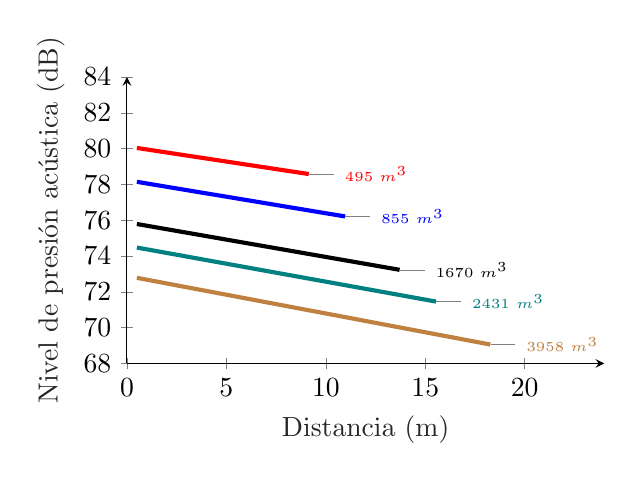
\begin{tikzpicture}

\begin{axis}[%
width=0.5\textwidth,
height=0.3\textwidth,
at={(0\textwidth,0\textwidth)},
scale only axis,
xmin=0,
xmax=24,
xlabel style={font=\color{white!15!black}},
xlabel={Distancia (m)},
ymin=68,
ymax=84,
ytick distance=2,
axis y line=left,
axis x line=bottom,
cycle list name=color list,
ylabel style={font=\color{white!15!black}},
ylabel={Nivel de presión acústica (dB)},
axis background/.style={fill=white},
legend style={legend cell align=left, align=left, draw=white!15!black}
]

% Campos utiles

% 1
\addplot+[ line width=1.5,domain=0.5:9.14, samples=10,every node/.style={xshift=-4pt}]
{10*log10(1.0337e+12 * ( (4*0.0026389378)/(512*(-ln(1-0.1176))) * e^(-(13.82*((x/343)+0.05)*1.195 / 1.24))*1.175))} node [pos=1,pin=0:{\tiny{495 $m^3$}}] {};

% 1.2
\addplot+[ line width=1.5,domain=0.5:10.97, samples=10,every node/.style={xshift=-4pt}]
{10*log10(1.0337e+12 * ( (4*0.0026389378)/(737*(-ln(1-0.1176))) * e^(-(13.82*((x/343)+0.05)*1.309 / 1.24))*1.168))} node [pos=1,pin=0:{\tiny{855 $m^3$}}] {};

% 1.5
\addplot+[ line width=1.5,domain=0.5:13.71, samples=10,every node/.style={xshift=-4pt}]
{10*log10(1.0337e+12 * ( (4*0.0026389378)/(1152*(-ln(1-0.1176))) * e^(-(13.82*((x/343)+0.05)*1.373 / 1.24))*1.101))} node [pos=1,pin=0:{\tiny{1670 $m^3$}}] {};

%% 1.7
\addplot[line width=1.5,color=teal, domain=0.5:15.54, samples=10,every node/.style={xshift=-4pt}]
{10*log10(1.0337e+12 * ( (4*0.0026389378)/(1479*(-ln(1-0.1176))) * e^(-(13.82*((x/343)+0.05)*1.422 / 1.24))*1.074))} node [pos=1,pin=0:{\tiny{2431 $m^3$}}] {};

% 20
\addplot+[ line width=1.5,domain=0.5:18.27, samples=10,every node/.style={xshift=-4pt}]
{10*log10(1.0337e+12 * ( (4*0.0026389378)/(2048*(-ln(1-0.1176))) * e^(-(13.82*((x/343)+0.05)*1.486 / 1.24))*1.045))} node [pos=1,pin=0:{\tiny{3958 $m^3$}}] {};


\end{axis}
\end{tikzpicture}%



%
    \caption{OP/S003}%
\end{figure}%

\subsection{Barras}
Otro ejemplo es la gráfica de barras:
\begin{lstlisting}[style=Latex-color]
\begin{figure}[ht]
\centering
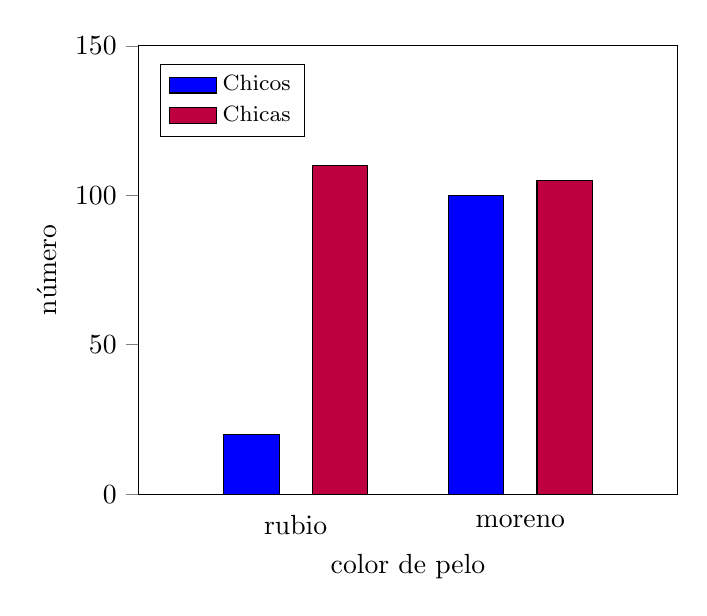
\begin{tikzpicture}
	\begin{axis}[
	    ybar=12pt,
	    ymin=0,ymax=150,
	    xtick=data,
	    enlarge x limits={abs=2cm},
	    symbolic x coords={rubio, moreno},
	    bar width = 20pt,
	    ylabel= número,
	    xlabel= color de pelo,
	        ytick align=outside,
	        ytick pos=left,
	        major x tick style = transparent,
	        legend style={at={(0.04,0.96)},anchor=north west, font=\footnotesize, legend cell align=left,},
	        ]
	    \addplot[ybar,fill=blue, area legend] coordinates {
	        (rubio,20)
	        (moreno,100)};
	    \addplot[ybar,fill=purple, area legend] coordinates {
	        (rubio,110)
	        (moreno,105)};
	 \legend{Chicos, Chicas}
	\end{axis}
\end{tikzpicture}
\caption{Gráfica barras.}
\end{figure}
\end{lstlisting}

El resultado es el siguiente:

\begin{figure}[ht]
\centering
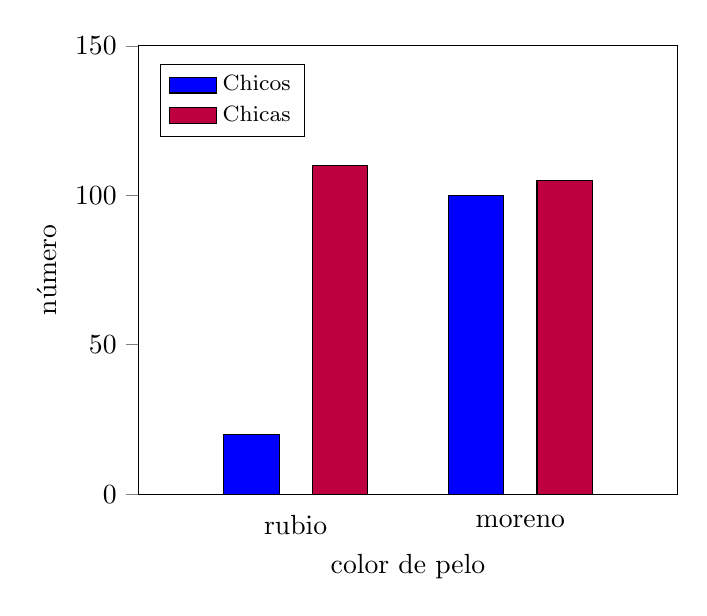
\begin{tikzpicture}
	\begin{axis}[
	    ybar=12pt,
	    ymin=0,ymax=150,
	    xtick=data,
	    enlarge x limits={abs=2cm},
	    symbolic x coords={rubio, moreno},
	    bar width = 20pt,
	    ylabel= número,
	    xlabel= color de pelo,
	        ytick align=outside,
	        ytick pos=left,
	        major x tick style = transparent,
	        legend style={at={(0.04,0.96)},anchor=north west, font=\footnotesize, legend cell align=left,},
	        ]
	    \addplot[ybar,fill=blue, area legend] coordinates {
	        (rubio,20)
	        (moreno,100)};
	    \addplot[ybar,fill=purple, area legend] coordinates {
	        (rubio,110)
	        (moreno,105)};
	 \legend{Chicos, Chicas}
	\end{axis}
\end{tikzpicture}
\caption{Gráfica barras.}
\end{figure}
\FloatBarrier

\subsection{Polar}
Un ejemplo de gráfica polar semicircular (ver archivo archivos/ejemplos/polarnorm.tex):

\begin{figure}[H]
    	\centering%
         {\scalefont{0.8}%
    %%%%%%%%%%%%%%%%%%%%%%%%%%%%%%%%%%%%%%%%%%%%%%%%%%%%%%%%%%%%%%%%%%%%%%%%
% Plantilla TFG/TFM
% Escuela Politécnica Superior de la Universidad de Alicante
% Realizado por: Jose Manuel Requena Plens
% Contacto: info@jmrplens.com / Telegram:@jmrplens
%%%%%%%%%%%%%%%%%%%%%%%%%%%%%%%%%%%%%%%%%%%%%%%%%%%%%%%%%%%%%%%%%%%%%%%%


\begin{tikzpicture}
\begin{polaraxis}[
	width=0.7\textwidth,
	height=0.7\textwidth,
   	ymin=-24,ymax=0,
   	xmin=-90,xmax=90,
   	xtick={-90,-75,...,90},
   	ytick={-24,-18,...,0},
   	minor y tick num=1,
   	ytick style={yshift=-4.63cm},
   	xticklabel=$\pgfmathprintnumber{\tick}^\circ$,
   	xticklabel style={inner xsep=1pt,ellipse,anchor=\tick-90},
   	yticklabel style={xshift=-0.3cm,yshift=-0.3cm},
   	rotate=90,
   	y coord trafo/.code=\pgfmathparse{#1+24},
   	y coord inv trafo/.code=\pgfmathparse{#1-24},
  	ylabel={Atenuación (dBV)},
   	y label style={at={(0.42,-0.3)}},
    every axis legend/.append style={at={(1.2,0)},anchor=north},
   	legend columns=4,
   	cycle list name=color list,
  	grid=both,
]
%%%%
% DATOS
%%%%

% 125 Hz
\addplot+ [no markers, thick] table [row sep=crcr] {
-90	-1.72467814939056\\
-80	-1.39502194748928\\
-70	-1.21429283845364\\
-60	-1.00637477945158\\
-50	-0.840171759843390\\
-40	-0.513117825581858\\
-30	-0.312245425134396\\
-20	-0.174766911961633\\
-10	-0.0693431271095548\\
0	0\\
10	-0.0693431271095548\\
20	-0.174766911961633\\
30	-0.312245425134396\\
40	-0.513117825581858\\
50	-0.840171759843390\\
60	-1.00637477945158\\
70	-1.21429283845364\\
80	-1.39502194748928\\
90	-1.72467814939056\\
};
\addlegendentry{125 Hz}

% 250 Hz
\addplot+ [no markers, thick] table [row sep=crcr] {
-90	-2.93647985014495\\
-80	-2.58924713825609\\
-70	-2.07154743573673\\
-60	-1.58004347746668\\
-50	-1.18692289277002\\
-40	-0.831096645385170\\
-30	-0.520252849633241\\
-20	-0.290340966177958\\
-10	-0.125751595259928\\
0	0\\
10	-0.125751595259928\\
20	-0.290340966177958\\
30	-0.520252849633241\\
40	-0.831096645385170\\
50	-1.18692289277002\\
60	-1.58004347746668\\
70	-2.07154743573673\\
80	-2.58924713825609\\
90	-2.93647985014495\\
};
\addlegendentry{250 Hz}

% 500 Hz
\addplot+ [no markers, thick] table [row sep=crcr] {
-90	-6.09247981547998\\
-80	-4.92970035404602\\
-70	-3.94022779907609\\
-60	-3.04724262203246\\
-50	-2.20250965801318\\
-40	-1.51751670631493\\
-30	-0.901656083415322\\
-20	-0.430295873745550\\
-10	-0.137302043547450\\
0	0\\
10	-0.137302043547450\\
20	-0.430295873745550\\
30	-0.901656083415322\\
40	-1.51751670631493\\
50	-2.20250965801318\\
60	-3.04724262203246\\
70	-3.94022779907609\\
80	-4.92970035404602\\
90	-6.09247981547998\\
};
\addlegendentry{500 Hz}

% 1000 Hz
\addplot+ [no markers, thick] table [row sep=crcr] {
-90	-7.56789211935512\\
-80	-6.62816595706798\\
-70	-5.52277371644042\\
-60	-4.33467545812354\\
-50	-3.13339535257511\\
-40	-2.05909345347580\\
-30	-1.17203420486137\\
-20	-0.523179334693538\\
-10	-0.128596775989607\\
0	0\\
10	-0.128596775989607\\
20	-0.523179334693538\\
30	-1.17203420486137\\
40	-2.05909345347580\\
50	-3.13339535257511\\
60	-4.33467545812354\\
70	-5.52277371644042\\
80	-6.62816595706798\\
90	-7.56789211935512\\
};
\addlegendentry{1 kHz}

% 2000 Hz
\addplot+ [no markers, thick] table [row sep=crcr] {
-90	-14.4940605430080\\
-80	-12.7515170649147\\
-70	-10.9391538310668\\
-60	-9.13813062972114\\
-50	-7.31396133207484\\
-40	-5.44124573776644\\
-30	-3.54658907253479\\
-20	-1.91024948494566\\
-10	-0.704464176648823\\
0	0\\
10	-0.704464176648823\\
20	-1.91024948494566\\
30	-3.54658907253479\\
40	-5.44124573776644\\
50	-7.31396133207484\\
60	-9.13813062972114\\
70	-10.9391538310668\\
80	-12.7515170649147\\
90	-14.4940605430080\\
};
\addlegendentry{2 kHz}

% 4000 Hz
\addplot+ [no markers, thick] table [row sep=crcr] {
-90	-20.8595379753136\\
-80	-19.5111125476763\\
-70	-17.5530334315451\\
-60	-15.1562865020723\\
-50	-12.6153094614475\\
-40	-9.78583047231908\\
-30	-6.34807022561957\\
-20	-3.07890709456410\\
-10	-0.920648439706582\\
0	0\\
10	-0.920648439706582\\
20	-3.07890709456410\\
30	-6.34807022561957\\
40	-9.78583047231908\\
50	-12.6153094614475\\
60	-15.1562865020723\\
70	-17.5530334315451\\
80	-19.5111125476763\\
90	-20.8595379753136\\
};
\addlegendentry{4 kHz}

% 8000 Hz
\addplot+ [no markers, thick] table [row sep=crcr] {
-90	-19.8608838454044\\
-80	-17.8504412710498\\
-70	-14.6995990848335\\
-60	-12.7200970148256\\
-50	-10.7405694231973\\
-40	-8.26676493005069\\
-30	-4.30385837835709\\
-20	-2.28439452050384\\
-10	-1.25666726464311\\
0	0\\
10	-1.25666726464311\\
20	-2.28439452050384\\
30	-4.30385837835709\\
40	-8.26676493005069\\
50	-10.7405694231973\\
60	-12.7200970148256\\
70	-14.6995990848335\\
80	-17.8504412710498\\
90	-19.8608838454044\\
};
\addlegendentry{8 kHz}

% 16000 Hz
\addplot+ [no markers, thick] table [row sep=crcr] {
-90	-13.2702037690998\\
-80	-13.0567210721723\\
-70	-11.6584528874959\\
-60	-10.0279714036086\\
-50	-9.30230549595443\\
-40	-5.30129835593380\\
-30	-5.79648449690136\\
-20	-6.18064845743399\\
-10	-3.22991472126657\\
0	0\\
10	-3.22991472126657\\
20	-6.18064845743399\\
30	-5.79648449690136\\
40	-5.30129835593380\\
50	-9.30230549595443\\
60	-10.0279714036086\\
70	-11.6584528874959\\
80	-13.0567210721723\\
90	-13.2702037690998\\
};
\addlegendentry{16 kHz}


\end{polaraxis}

\end{tikzpicture}%%
    }
    \caption{Directividad normalizada del altavoz (0 dBV en el eje).}\label{norma}
\end{figure}


\section{Importados de MATLAB}
\label{impmatlab}
Gracias a la herramienta \textit{matlab2tikz} (\url{https://es.mathworks.com/matlabcentral/fileexchange/22022-matlab2tikz-matlab2tikz}) se pueden exportar las gráficas de cualquier tipo de Matlab a latex.
Después de incluir los archivos de \textit{matlab2tikz} se debe escribir una llamada después de crear la figura tal que:

\begin{lstlisting}[style=Matlab-color,caption={Ejemplo de llamada a matlab2tikz}]
fig = plot(x,y);
matlab2tikz('figurehandle',fig,'NombreArchivo.tex','height','5cm','width','13.5cm','strict',true,'showHiddenStrings',true,'showInfo',false)
\end{lstlisting}

Y para utilizar el archivo generado por la función en este documento:
\begin{lstlisting}[style=Latex-color]
\begin{figure}[ht]
	\centering
	{\scalefont{0.8}% This file was created by matlab2tikz.
%
\definecolor{mycolor1}{rgb}{0.00000,1.00000,1.00000}%
%
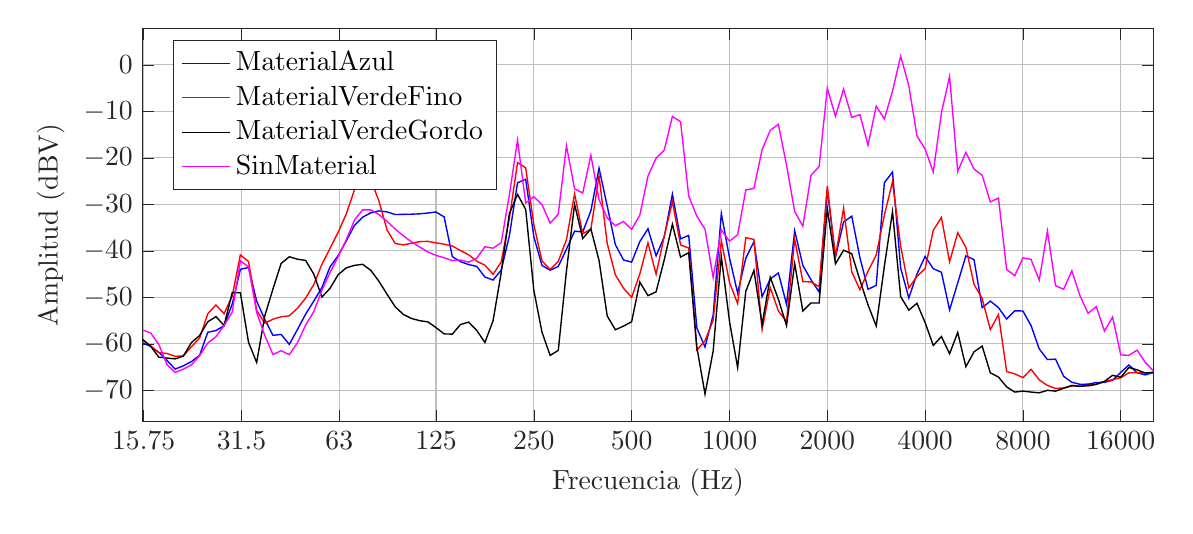
\begin{tikzpicture}

\begin{axis}[%
width=12.837cm,
height=5cm,
at={(0cm,0cm)},
scale only axis,
separate axis lines,
every outer x axis line/.append style={white!15!black},
every x tick label/.append style={font=\color{white!15!black}},
every x tick/.append style={white!15!black},
xmode=log,
xmin=15.625,
xmax=20158.736798318,
xtick={15.75,31.5,63,125,250,500,1000,2000,4000,8000,16000,24000},
xticklabels={{15.75},{31.5},{63},{125},{250},{500},{1000},{2000},{4000},{8000},{16000},{24000}},
xminorticks=true,
minor x tick num={3},
xlabel style={font=\color{white!15!black}},
xlabel={Frecuencia (Hz)},
every outer y axis line/.append style={white!15!black},
every y tick label/.append style={font=\color{white!15!black}},
every y tick/.append style={white!15!black},
ymin=-76.8103540908063,
ymax=7.89608497583378,
ytick={-70,-60,-50,-40,-30,-20,-10,0},
ylabel style={font=\color{white!15!black}},
ylabel={Amplitud (dBV)},
axis background/.style={fill=white},
xmajorgrids,
xminorgrids,
ymajorgrids,
grid style={solid},
minor grid style={dotted},
legend style={at={(0.03,0.97)}, anchor=north west, legend cell align=left, align=left, draw=white!15!black}
]
\addplot [color=blue, line width=0.5pt]
  table[row sep=crcr]{%
15.625	-59.82445\\
16.554110849364	-60.5623842620438\\
17.538469504834	-61.8453599337536\\
18.5813611719175	-63.5771407909652\\
19.6862664046074	-65.4392\\
20.8568727214068	-64.7401066715843\\
22.0970869120796	-63.8280672771138\\
23.4110480761981	-62.4796867506898\\
24.8031414370031	-57.5235393587445\\
26.2780129766786	-57.1510284649747\\
27.8405849418856	-56.1120339592741\\
29.4960722713029	-51.4584375460028\\
31.25	-43.9775628086098\\
33.108221698728	-43.5775399935433\\
35.0769390096679	-50.8056912623702\\
37.162722343835	-54.7762319229848\\
39.3725328092148	-58.1818541033231\\
41.7137454428136	-57.9871674094596\\
44.1941738241592	-60.131686917752\\
46.8220961523963	-56.9321010863531\\
49.6062828740062	-53.6269734128779\\
52.5560259533572	-50.8326803688349\\
55.6811698837712	-47.9044516763833\\
58.9921445426058	-43.4540614843463\\
62.5	-41.0088562276629\\
66.216443397456	-37.8454981965748\\
70.1538780193358	-34.5101536696686\\
74.3254446876701	-32.758999578223\\
78.7450656184296	-31.8221380801992\\
83.4274908856271	-31.4018682790007\\
88.3883476483184	-31.6205768805081\\
93.6441923047926	-32.1910113608511\\
99.2125657480125	-32.146745758715\\
105.112051906714	-32.1162035706091\\
111.362339767542	-32.0351296667358\\
117.984289085212	-31.8593374930549\\
125	-31.6438781217507\\
132.432886794912	-32.7077285823639\\
140.307756038672	-41.2380463075868\\
148.65088937534	-42.3286171523452\\
157.490131236859	-42.9588375664898\\
166.854981771254	-43.3416748711169\\
176.776695296637	-45.6421692384549\\
187.288384609585	-46.2756368008904\\
198.425131496025	-44.1520572452639\\
210.224103813429	-36.7562071223667\\
222.724679535085	-25.3615471609834\\
235.968578170423	-24.5871544187069\\
250	-36.9591372808033\\
264.865773589824	-43.147777613225\\
280.615512077343	-44.1738417685541\\
297.30177875068	-43.3530316256479\\
314.980262473718	-39.6469484745674\\
333.709963542509	-35.7621654522761\\
353.553390593274	-35.9408492154802\\
374.57676921917	-31.3873624257484\\
396.85026299205	-22.2157600934004\\
420.448207626857	-30.3268893562579\\
445.44935907017	-38.661267780467\\
471.937156340847	-41.9608541996203\\
500	-42.4233556402969\\
529.731547179648	-38.0294467540743\\
561.231024154687	-35.2495707063382\\
594.603557501361	-41.0788126861199\\
629.960524947437	-36.9611736331159\\
667.419927085017	-27.8036460694195\\
707.106781186547	-37.4246421028473\\
749.153538438341	-36.6736669360865\\
793.7005259841	-56.6093466744553\\
840.896415253715	-60.6854087092917\\
890.898718140339	-53.7923826138654\\
943.874312681693	-31.965259614882\\
1000	-41.4806385598563\\
1059.4630943593	-49.0691867123825\\
1122.46204830937	-41.5852844720362\\
1189.20711500272	-38.0368734949954\\
1259.92104989487	-49.8662236912185\\
1334.83985417003	-46.0616368809841\\
1414.2135623731	-44.7653335346495\\
1498.30707687668	-51.5065289570559\\
1587.4010519682	-35.6526112530488\\
1681.79283050743	-43.1342117855054\\
1781.79743628068	-46.2182887953753\\
1887.74862536339	-48.8673999243209\\
2000	-26.7690224183847\\
2118.92618871859	-41.3181000867668\\
2244.92409661875	-33.7917238250563\\
2378.41423000544	-32.5463108508702\\
2519.84209978975	-41.4721274862615\\
2669.67970834007	-48.2641692316123\\
2828.42712474619	-47.4314835648184\\
2996.61415375336	-25.3484775993174\\
3174.8021039364	-23.0465733116748\\
3363.58566101486	-43.6874762505469\\
3563.59487256136	-50.1366159423142\\
3775.49725072677	-44.9838149162718\\
4000	-41.201339624147\\
4237.85237743718	-43.8424573289536\\
4489.84819323749	-44.6017637320515\\
4756.82846001088	-52.7088030381003\\
5039.68419957949	-46.9012281486801\\
5339.35941668014	-41.0810782256828\\
5656.85424949238	-41.8854684412556\\
5993.22830750673	-52.2321725759016\\
6349.6042078728	-50.8166988416389\\
6727.17132202972	-52.2123476191788\\
7127.18974512272	-54.6853592109235\\
7550.99450145355	-52.9011604035292\\
8000	-52.9404553936464\\
8475.70475487436	-56.0951609030491\\
8979.69638647498	-61.1026839941301\\
9513.65692002177	-63.3820382977075\\
10079.368399159	-63.3021538084351\\
10678.7188333603	-66.9975797930797\\
11313.7084989848	-68.2808725877187\\
11986.4566150135	-68.7092813281996\\
12699.2084157456	-68.6816428164156\\
13454.3426440594	-68.3295378979568\\
14254.3794902454	-68.2956064680681\\
15101.9890029071	-67.832346962215\\
16000	-66.1488584556794\\
16951.4095097487	-64.5515563892345\\
17959.39277295	-66.2310858769382\\
19027.3138400435	-66.6868616467929\\
20158.736798318	-66.206951771162\\
};
\addlegendentry{MaterialAzul}

\addplot [color=red, line width=0.5pt]
  table[row sep=crcr]{%
15.625	-59.19615\\
16.554110849364	-60.4758401197422\\
17.538469504834	-61.901396505329\\
18.5813611719175	-62.0797319785541\\
19.6862664046074	-62.6988\\
20.8568727214068	-62.6165353275886\\
22.0970869120796	-60.6368804056736\\
23.4110480761981	-58.7628282862501\\
24.8031414370031	-53.5412438017337\\
26.2780129766786	-51.6384009922331\\
27.8405849418856	-53.5071809202347\\
29.4960722713029	-49.7199983161259\\
31.25	-40.8687363671337\\
33.108221698728	-42.305478953612\\
35.0769390096679	-52.8127397529563\\
37.162722343835	-55.5615931008179\\
39.3725328092148	-54.7062248399483\\
41.7137454428136	-54.1865533882828\\
44.1941738241592	-53.9687472439094\\
46.8220961523963	-52.3746981661219\\
49.6062828740062	-50.175536919246\\
52.5560259533572	-47.2757670280218\\
55.6811698837712	-42.9136417155744\\
58.9921445426058	-39.4577835838755\\
62.5	-35.977781131089\\
66.216443397456	-32.0287595831997\\
70.1538780193358	-26.859138430704\\
74.3254446876701	-23.5138223410267\\
78.7450656184296	-24.6789065147145\\
83.4274908856271	-29.2914472283602\\
88.3883476483184	-35.5456855246057\\
93.6441923047926	-38.4196962749671\\
99.2125657480125	-38.7208351109208\\
105.112051906714	-38.3560680143838\\
111.362339767542	-38.0129601333831\\
117.984289085212	-37.9586922428017\\
125	-38.2746442985451\\
132.432886794912	-38.5680827068538\\
140.307756038672	-38.9487275790866\\
148.65088937534	-39.9418082905037\\
157.490131236859	-40.8370996613296\\
166.854981771254	-42.2221732181026\\
176.776695296637	-43.0799629198218\\
187.288384609585	-45.0639834460553\\
198.425131496025	-42.3955435739198\\
210.224103813429	-32.9664436186507\\
222.724679535085	-21.014020510176\\
235.968578170423	-22.1207001985688\\
250	-34.3804918874655\\
264.865773589824	-42.1589405956387\\
280.615512077343	-43.9955479985442\\
297.30177875068	-42.2526062402211\\
314.980262473718	-37.6102060538754\\
333.709963542509	-27.7307065397205\\
353.553390593274	-36.3476292630841\\
374.57676921917	-35.3285325552507\\
396.85026299205	-23.909551502887\\
420.448207626857	-38.4192944329836\\
445.44935907017	-45.1775867907933\\
471.937156340847	-48.0365164882642\\
500	-50.0129423561998\\
529.731547179648	-44.9703926258222\\
561.231024154687	-38.2735269338767\\
594.603557501361	-45.0415844154744\\
629.960524947437	-36.8302928772219\\
667.419927085017	-29.4340532872101\\
707.106781186547	-38.7307713465337\\
749.153538438341	-39.3964196430224\\
793.7005259841	-61.3440115615457\\
840.896415253715	-59.3244862211819\\
890.898718140339	-54.9145405450293\\
943.874312681693	-37.7865556153937\\
1000	-46.79124761546\\
1059.4630943593	-51.3497729083625\\
1122.46204830937	-37.153598550838\\
1189.20711500272	-37.5507639581768\\
1259.92104989487	-56.9338074452588\\
1334.83985417003	-47.9012681154996\\
1414.2135623731	-52.9553016631441\\
1498.30707687668	-55.1738616862925\\
1587.4010519682	-37.5057700354591\\
1681.79283050743	-46.6066693513474\\
1781.79743628068	-46.6896979706392\\
1887.74862536339	-47.7032390735606\\
2000	-26.0320439894176\\
2118.92618871859	-41.3137465050699\\
2244.92409661875	-30.8298541081918\\
2378.41423000544	-44.496254678482\\
2519.84209978975	-48.3751258261709\\
2669.67970834007	-44.3805239761309\\
2828.42712474619	-40.8912353753558\\
2996.61415375336	-32.3339101743683\\
3174.8021039364	-25.1344010767185\\
3363.58566101486	-38.9887687971321\\
3563.59487256136	-47.9894796761595\\
3775.49725072677	-45.4799526214346\\
4000	-43.8434545595259\\
4237.85237743718	-35.5920294193788\\
4489.84819323749	-32.819844689661\\
4756.82846001088	-42.3539734847047\\
5039.68419957949	-36.1213846668969\\
5339.35941668014	-39.2326411780269\\
5656.85424949238	-47.2292598354812\\
5993.22830750673	-50.2601819195157\\
6349.6042078728	-56.9575923846714\\
6727.17132202972	-53.6911046049363\\
7127.18974512272	-65.9629427801802\\
7550.99450145355	-66.4643543317632\\
8000	-67.2789827829873\\
8475.70475487436	-65.4968201055031\\
8979.69638647498	-67.7538648896841\\
9513.65692002177	-68.9515236625436\\
10079.368399159	-69.609644625656\\
10678.7188333603	-69.4946963076361\\
11313.7084989848	-68.9235995478426\\
11986.4566150135	-69.0920877977121\\
12699.2084157456	-69.0788594566697\\
13454.3426440594	-68.7506219152814\\
14254.3794902454	-68.0952602567396\\
15101.9890029071	-67.7220558117344\\
16000	-67.2968401658589\\
16951.4095097487	-66.2507837637718\\
17959.39277295	-66.1952921165776\\
19027.3138400435	-66.2845535682028\\
20158.736798318	-66.2431030573677\\
};
\addlegendentry{MaterialVerdeFino}

\addplot [color=black, line width=0.5pt]
  table[row sep=crcr]{%
15.625	-59.0501\\
16.554110849364	-60.5481459724334\\
17.538469504834	-62.8737034867959\\
18.5813611719175	-63.0653491134085\\
19.6862664046074	-63.2439\\
20.8568727214068	-62.647923280359\\
22.0970869120796	-59.7296877694629\\
23.4110480761981	-58.2107719822048\\
24.8031414370031	-55.2728350225112\\
26.2780129766786	-54.1500091439273\\
27.8405849418856	-56.0570014986231\\
29.4960722713029	-49.0103259775126\\
31.25	-49.0100345661345\\
33.108221698728	-59.6650430567775\\
35.0769390096679	-64.0110522942114\\
37.162722343835	-53.9521428678289\\
39.3725328092148	-48.2086200564461\\
41.7137454428136	-42.712594474368\\
44.1941738241592	-41.2714765087534\\
46.8220961523963	-41.7987201570495\\
49.6062828740062	-42.0507436945294\\
52.5560259533572	-44.982722192644\\
55.6811698837712	-49.9507907604182\\
58.9921445426058	-48.0643265760432\\
62.5	-45.1242785513276\\
66.216443397456	-43.6464175968642\\
70.1538780193358	-43.1252659616118\\
74.3254446876701	-42.8959424161612\\
78.7450656184296	-44.1868508520227\\
83.4274908856271	-46.5601173245115\\
88.3883476483184	-49.3568449622491\\
93.6441923047926	-52.0515121074992\\
99.2125657480125	-53.6834617815862\\
105.112051906714	-54.5590280069015\\
111.362339767542	-55.0262358707017\\
117.984289085212	-55.2811465539582\\
125	-56.5186733537943\\
132.432886794912	-57.8704431925443\\
140.307756038672	-57.9177569490739\\
148.65088937534	-55.8568407526673\\
157.490131236859	-55.3255067194691\\
166.854981771254	-57.1235281279484\\
176.776695296637	-59.7153653919227\\
187.288384609585	-55.0446832882348\\
198.425131496025	-44.6850934873909\\
210.224103813429	-31.9768034452654\\
222.724679535085	-27.8451073069786\\
235.968578170423	-31.0866597302841\\
250	-48.5008216163439\\
264.865773589824	-57.4858808267551\\
280.615512077343	-62.4896852938823\\
297.30177875068	-61.4258686006565\\
314.980262473718	-44.3408329903174\\
333.709963542509	-30.0072398949372\\
353.553390593274	-37.3436080312732\\
374.57676921917	-35.2872068103096\\
396.85026299205	-42.0617640773635\\
420.448207626857	-54.0018459158019\\
445.44935907017	-56.9814413980227\\
471.937156340847	-56.1957360933461\\
500	-55.2472162010321\\
529.731547179648	-46.7204322842484\\
561.231024154687	-49.6382092063127\\
594.603557501361	-48.8202129999924\\
629.960524947437	-41.9134070439017\\
667.419927085017	-34.2658048087529\\
707.106781186547	-41.3477365160178\\
749.153538438341	-40.3949844671083\\
793.7005259841	-60.7225116106643\\
840.896415253715	-70.8103540908063\\
890.898718140339	-61.5425686950677\\
943.874312681693	-41.2653288040076\\
1000	-55.1412465569446\\
1059.4630943593	-65.0993335283221\\
1122.46204830937	-48.7310378648667\\
1189.20711500272	-44.1999544789567\\
1259.92104989487	-55.8276465112632\\
1334.83985417003	-45.7030741073327\\
1414.2135623731	-50.4275766639819\\
1498.30707687668	-56.0995867094959\\
1587.4010519682	-42.7288687592806\\
1681.79283050743	-52.9406454617406\\
1781.79743628068	-51.2092369894416\\
1887.74862536339	-51.2107739581227\\
2000	-30.8976239663764\\
2118.92618871859	-42.7957999734761\\
2244.92409661875	-39.867639055906\\
2378.41423000544	-40.622428502866\\
2519.84209978975	-46.297109640538\\
2669.67970834007	-51.6510753146547\\
2828.42712474619	-56.1684424549805\\
2996.61415375336	-43.3239161711086\\
3174.8021039364	-31.563333108932\\
3363.58566101486	-49.8237940579162\\
3563.59487256136	-52.7698764192602\\
3775.49725072677	-51.2740685144341\\
4000	-55.4509748853548\\
4237.85237743718	-60.3517496524667\\
4489.84819323749	-58.4394780093032\\
4756.82846001088	-62.1432337016279\\
5039.68419957949	-57.5645773082218\\
5339.35941668014	-64.9344581438538\\
5656.85424949238	-61.7344247927045\\
5993.22830750673	-60.4913901744954\\
6349.6042078728	-66.250132868323\\
6727.17132202972	-67.1462149783166\\
7127.18974512272	-69.2770440952632\\
7550.99450145355	-70.3858798182754\\
8000	-70.1773540679127\\
8475.70475487436	-70.3814839627002\\
8979.69638647498	-70.5496860924335\\
9513.65692002177	-70.0105465696835\\
10079.368399159	-70.178826585874\\
10678.7188333603	-69.5630650672476\\
11313.7084989848	-69.0340966967485\\
11986.4566150135	-69.1596385340084\\
12699.2084157456	-68.9411167962604\\
13454.3426440594	-68.691230739146\\
14254.3794902454	-68.0981739116805\\
15101.9890029071	-66.7728745251338\\
16000	-67.20043767062\\
16951.4095097487	-65.1044221489216\\
17959.39277295	-65.596322314587\\
19027.3138400435	-66.2803507242832\\
20158.736798318	-66.1272732833845\\
};
\addlegendentry{MaterialVerdeGordo}

\addplot [color=mycolor1, line width=0.5pt]
  table[row sep=crcr]{%
15.625	-57.0491\\
16.554110849364	-57.6577400860243\\
17.538469504834	-60.1577461651464\\
18.5813611719175	-64.4723155301311\\
19.6862664046074	-66.15515\\
20.8568727214068	-65.4508565703522\\
22.0970869120796	-64.5352879365434\\
23.4110480761981	-62.5722791910146\\
24.8031414370031	-59.8217365780248\\
26.2780129766786	-58.4778394106456\\
27.8405849418856	-56.1016081859342\\
29.4960722713029	-53.1960678901614\\
31.25	-42.1319921685267\\
33.108221698728	-43.4553452207726\\
35.0769390096679	-53.2600454559127\\
37.162722343835	-58.2230527846992\\
39.3725328092148	-62.3138206894883\\
41.7137454428136	-61.4729842893297\\
44.1941738241592	-62.3404413664062\\
46.8220961523963	-59.7713655312374\\
49.6062828740062	-55.9978810660399\\
52.5560259533572	-53.0931025874956\\
55.6811698837712	-48.4879111005475\\
58.9921445426058	-44.6737822644256\\
62.5	-41.2483734494907\\
66.216443397456	-37.5659885888276\\
70.1538780193358	-33.3763408930803\\
74.3254446876701	-31.1730867960601\\
78.7450656184296	-31.1760198533411\\
83.4274908856271	-32.1942100727774\\
88.3883476483184	-33.660597259321\\
93.6441923047926	-35.3320865133628\\
99.2125657480125	-36.7688395629296\\
105.112051906714	-38.0742321196065\\
111.362339767542	-39.1857007549765\\
117.984289085212	-40.2216604012084\\
125	-40.9752709135297\\
132.432886794912	-41.4911631794347\\
140.307756038672	-42.0845009497682\\
148.65088937534	-41.9652476231725\\
157.490131236859	-42.4395475230036\\
166.854981771254	-41.5726934826067\\
176.776695296637	-39.1186549394196\\
187.288384609585	-39.4337070045907\\
198.425131496025	-38.2507499398096\\
210.224103813429	-27.9397795564285\\
222.724679535085	-16.1766474272004\\
235.968578170423	-29.72031524715\\
250	-28.3627651969203\\
264.865773589824	-30.0450446666323\\
280.615512077343	-34.0390110745634\\
297.30177875068	-32.1223470220443\\
314.980262473718	-17.3811846319238\\
333.709963542509	-26.6764650376163\\
353.553390593274	-27.5511784985874\\
374.57676921917	-19.4478252698716\\
396.85026299205	-29.001264295923\\
420.448207626857	-32.8992924354827\\
445.44935907017	-34.6005912785462\\
471.937156340847	-33.6948405249946\\
500	-35.3790180734319\\
529.731547179648	-32.3280895557714\\
561.231024154687	-23.916767635231\\
594.603557501361	-20.0421927166081\\
629.960524947437	-18.3399010991622\\
667.419927085017	-11.0761845904328\\
707.106781186547	-12.2156347315298\\
749.153538438341	-28.2241666522327\\
793.7005259841	-32.5356063174604\\
840.896415253715	-35.3276266753434\\
890.898718140339	-45.7523322001687\\
943.874312681693	-35.4801475828069\\
1000	-37.9131864983456\\
1059.4630943593	-36.5408696190504\\
1122.46204830937	-26.9090614647777\\
1189.20711500272	-26.5554164163196\\
1259.92104989487	-18.2348810829384\\
1334.83985417003	-14.0723172842119\\
1414.2135623731	-12.7848786602511\\
1498.30707687668	-21.5440462957906\\
1587.4010519682	-31.5417666251209\\
1681.79283050743	-34.7005769511542\\
1781.79743628068	-23.7476801011984\\
1887.74862536339	-21.876286190819\\
2000	-5.02239335516242\\
2118.92618871859	-11.0211823642914\\
2244.92409661875	-5.21109808728585\\
2378.41423000544	-11.2948092845673\\
2519.84209978975	-10.6972799671187\\
2669.67970834007	-17.2733306879063\\
2828.42712474619	-8.8542246222065\\
2996.61415375336	-11.6599052832243\\
3174.8021039364	-5.63762732056441\\
3363.58566101486	1.89608497583378\\
3563.59487256136	-4.44752681282801\\
3775.49725072677	-15.2836256859219\\
4000	-18.1092239316893\\
4237.85237743718	-23.0457911756979\\
4489.84819323749	-10.3136636223751\\
4756.82846001088	-2.47118821728687\\
5039.68419957949	-22.9008564436342\\
5339.35941668014	-18.808699198178\\
5656.85424949238	-22.4030769288758\\
5993.22830750673	-23.7492487981603\\
6349.6042078728	-29.4910947963741\\
6727.17132202972	-28.6389901928041\\
7127.18974512272	-44.0019622979657\\
7550.99450145355	-45.3416258722268\\
8000	-41.5004841172652\\
8475.70475487436	-41.8544902557376\\
8979.69638647498	-46.3081962019953\\
9513.65692002177	-35.7206561393855\\
10079.368399159	-47.505258507613\\
10678.7188333603	-48.250954042689\\
11313.7084989848	-44.2800890053478\\
11986.4566150135	-49.6738256154224\\
12699.2084157456	-53.4390035491901\\
13454.3426440594	-52.0083953186444\\
14254.3794902454	-57.2428357619752\\
15101.9890029071	-54.2281517571219\\
16000	-62.3933852733234\\
16951.4095097487	-62.4823163951875\\
17959.39277295	-61.3655852903141\\
19027.3138400435	-63.9771653522834\\
20158.736798318	-65.800940990071\\
};
\addlegendentry{SinMaterial}

\end{axis}
\end{tikzpicture}% }
	\caption{Ejemplo de gráfica obtenida con matlab2tikz.}
\end{figure}
\end{lstlisting}

\begin{figure}[ht]
	\centering
	{\scalefont{0.8}% This file was created by matlab2tikz.
%
\definecolor{mycolor1}{rgb}{0.00000,1.00000,1.00000}%
%
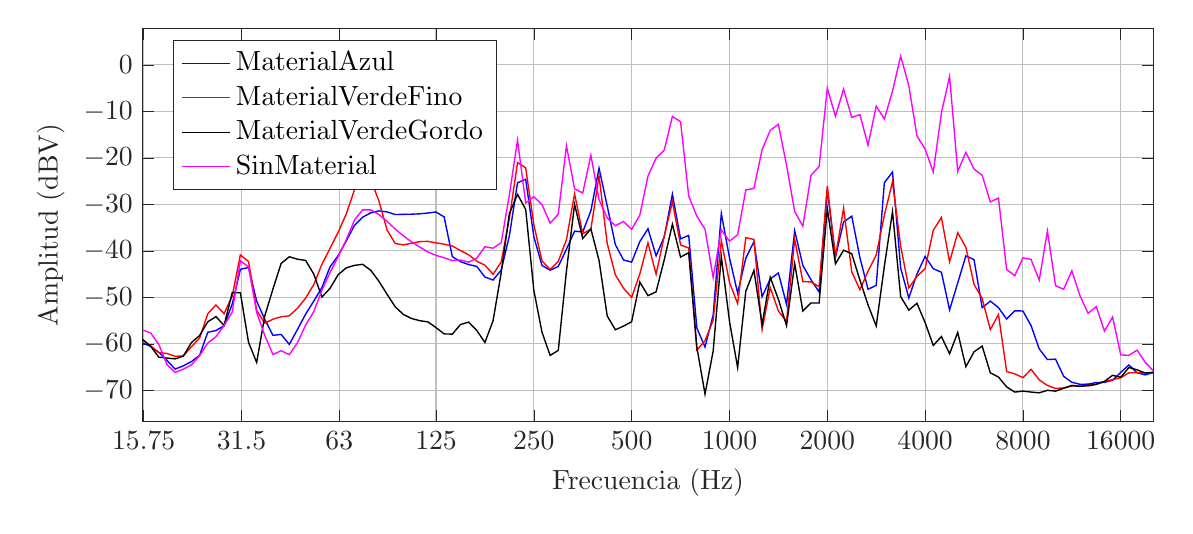
\begin{tikzpicture}

\begin{axis}[%
width=12.837cm,
height=5cm,
at={(0cm,0cm)},
scale only axis,
separate axis lines,
every outer x axis line/.append style={white!15!black},
every x tick label/.append style={font=\color{white!15!black}},
every x tick/.append style={white!15!black},
xmode=log,
xmin=15.625,
xmax=20158.736798318,
xtick={15.75,31.5,63,125,250,500,1000,2000,4000,8000,16000,24000},
xticklabels={{15.75},{31.5},{63},{125},{250},{500},{1000},{2000},{4000},{8000},{16000},{24000}},
xminorticks=true,
minor x tick num={3},
xlabel style={font=\color{white!15!black}},
xlabel={Frecuencia (Hz)},
every outer y axis line/.append style={white!15!black},
every y tick label/.append style={font=\color{white!15!black}},
every y tick/.append style={white!15!black},
ymin=-76.8103540908063,
ymax=7.89608497583378,
ytick={-70,-60,-50,-40,-30,-20,-10,0},
ylabel style={font=\color{white!15!black}},
ylabel={Amplitud (dBV)},
axis background/.style={fill=white},
xmajorgrids,
xminorgrids,
ymajorgrids,
grid style={solid},
minor grid style={dotted},
legend style={at={(0.03,0.97)}, anchor=north west, legend cell align=left, align=left, draw=white!15!black}
]
\addplot [color=blue, line width=0.5pt]
  table[row sep=crcr]{%
15.625	-59.82445\\
16.554110849364	-60.5623842620438\\
17.538469504834	-61.8453599337536\\
18.5813611719175	-63.5771407909652\\
19.6862664046074	-65.4392\\
20.8568727214068	-64.7401066715843\\
22.0970869120796	-63.8280672771138\\
23.4110480761981	-62.4796867506898\\
24.8031414370031	-57.5235393587445\\
26.2780129766786	-57.1510284649747\\
27.8405849418856	-56.1120339592741\\
29.4960722713029	-51.4584375460028\\
31.25	-43.9775628086098\\
33.108221698728	-43.5775399935433\\
35.0769390096679	-50.8056912623702\\
37.162722343835	-54.7762319229848\\
39.3725328092148	-58.1818541033231\\
41.7137454428136	-57.9871674094596\\
44.1941738241592	-60.131686917752\\
46.8220961523963	-56.9321010863531\\
49.6062828740062	-53.6269734128779\\
52.5560259533572	-50.8326803688349\\
55.6811698837712	-47.9044516763833\\
58.9921445426058	-43.4540614843463\\
62.5	-41.0088562276629\\
66.216443397456	-37.8454981965748\\
70.1538780193358	-34.5101536696686\\
74.3254446876701	-32.758999578223\\
78.7450656184296	-31.8221380801992\\
83.4274908856271	-31.4018682790007\\
88.3883476483184	-31.6205768805081\\
93.6441923047926	-32.1910113608511\\
99.2125657480125	-32.146745758715\\
105.112051906714	-32.1162035706091\\
111.362339767542	-32.0351296667358\\
117.984289085212	-31.8593374930549\\
125	-31.6438781217507\\
132.432886794912	-32.7077285823639\\
140.307756038672	-41.2380463075868\\
148.65088937534	-42.3286171523452\\
157.490131236859	-42.9588375664898\\
166.854981771254	-43.3416748711169\\
176.776695296637	-45.6421692384549\\
187.288384609585	-46.2756368008904\\
198.425131496025	-44.1520572452639\\
210.224103813429	-36.7562071223667\\
222.724679535085	-25.3615471609834\\
235.968578170423	-24.5871544187069\\
250	-36.9591372808033\\
264.865773589824	-43.147777613225\\
280.615512077343	-44.1738417685541\\
297.30177875068	-43.3530316256479\\
314.980262473718	-39.6469484745674\\
333.709963542509	-35.7621654522761\\
353.553390593274	-35.9408492154802\\
374.57676921917	-31.3873624257484\\
396.85026299205	-22.2157600934004\\
420.448207626857	-30.3268893562579\\
445.44935907017	-38.661267780467\\
471.937156340847	-41.9608541996203\\
500	-42.4233556402969\\
529.731547179648	-38.0294467540743\\
561.231024154687	-35.2495707063382\\
594.603557501361	-41.0788126861199\\
629.960524947437	-36.9611736331159\\
667.419927085017	-27.8036460694195\\
707.106781186547	-37.4246421028473\\
749.153538438341	-36.6736669360865\\
793.7005259841	-56.6093466744553\\
840.896415253715	-60.6854087092917\\
890.898718140339	-53.7923826138654\\
943.874312681693	-31.965259614882\\
1000	-41.4806385598563\\
1059.4630943593	-49.0691867123825\\
1122.46204830937	-41.5852844720362\\
1189.20711500272	-38.0368734949954\\
1259.92104989487	-49.8662236912185\\
1334.83985417003	-46.0616368809841\\
1414.2135623731	-44.7653335346495\\
1498.30707687668	-51.5065289570559\\
1587.4010519682	-35.6526112530488\\
1681.79283050743	-43.1342117855054\\
1781.79743628068	-46.2182887953753\\
1887.74862536339	-48.8673999243209\\
2000	-26.7690224183847\\
2118.92618871859	-41.3181000867668\\
2244.92409661875	-33.7917238250563\\
2378.41423000544	-32.5463108508702\\
2519.84209978975	-41.4721274862615\\
2669.67970834007	-48.2641692316123\\
2828.42712474619	-47.4314835648184\\
2996.61415375336	-25.3484775993174\\
3174.8021039364	-23.0465733116748\\
3363.58566101486	-43.6874762505469\\
3563.59487256136	-50.1366159423142\\
3775.49725072677	-44.9838149162718\\
4000	-41.201339624147\\
4237.85237743718	-43.8424573289536\\
4489.84819323749	-44.6017637320515\\
4756.82846001088	-52.7088030381003\\
5039.68419957949	-46.9012281486801\\
5339.35941668014	-41.0810782256828\\
5656.85424949238	-41.8854684412556\\
5993.22830750673	-52.2321725759016\\
6349.6042078728	-50.8166988416389\\
6727.17132202972	-52.2123476191788\\
7127.18974512272	-54.6853592109235\\
7550.99450145355	-52.9011604035292\\
8000	-52.9404553936464\\
8475.70475487436	-56.0951609030491\\
8979.69638647498	-61.1026839941301\\
9513.65692002177	-63.3820382977075\\
10079.368399159	-63.3021538084351\\
10678.7188333603	-66.9975797930797\\
11313.7084989848	-68.2808725877187\\
11986.4566150135	-68.7092813281996\\
12699.2084157456	-68.6816428164156\\
13454.3426440594	-68.3295378979568\\
14254.3794902454	-68.2956064680681\\
15101.9890029071	-67.832346962215\\
16000	-66.1488584556794\\
16951.4095097487	-64.5515563892345\\
17959.39277295	-66.2310858769382\\
19027.3138400435	-66.6868616467929\\
20158.736798318	-66.206951771162\\
};
\addlegendentry{MaterialAzul}

\addplot [color=red, line width=0.5pt]
  table[row sep=crcr]{%
15.625	-59.19615\\
16.554110849364	-60.4758401197422\\
17.538469504834	-61.901396505329\\
18.5813611719175	-62.0797319785541\\
19.6862664046074	-62.6988\\
20.8568727214068	-62.6165353275886\\
22.0970869120796	-60.6368804056736\\
23.4110480761981	-58.7628282862501\\
24.8031414370031	-53.5412438017337\\
26.2780129766786	-51.6384009922331\\
27.8405849418856	-53.5071809202347\\
29.4960722713029	-49.7199983161259\\
31.25	-40.8687363671337\\
33.108221698728	-42.305478953612\\
35.0769390096679	-52.8127397529563\\
37.162722343835	-55.5615931008179\\
39.3725328092148	-54.7062248399483\\
41.7137454428136	-54.1865533882828\\
44.1941738241592	-53.9687472439094\\
46.8220961523963	-52.3746981661219\\
49.6062828740062	-50.175536919246\\
52.5560259533572	-47.2757670280218\\
55.6811698837712	-42.9136417155744\\
58.9921445426058	-39.4577835838755\\
62.5	-35.977781131089\\
66.216443397456	-32.0287595831997\\
70.1538780193358	-26.859138430704\\
74.3254446876701	-23.5138223410267\\
78.7450656184296	-24.6789065147145\\
83.4274908856271	-29.2914472283602\\
88.3883476483184	-35.5456855246057\\
93.6441923047926	-38.4196962749671\\
99.2125657480125	-38.7208351109208\\
105.112051906714	-38.3560680143838\\
111.362339767542	-38.0129601333831\\
117.984289085212	-37.9586922428017\\
125	-38.2746442985451\\
132.432886794912	-38.5680827068538\\
140.307756038672	-38.9487275790866\\
148.65088937534	-39.9418082905037\\
157.490131236859	-40.8370996613296\\
166.854981771254	-42.2221732181026\\
176.776695296637	-43.0799629198218\\
187.288384609585	-45.0639834460553\\
198.425131496025	-42.3955435739198\\
210.224103813429	-32.9664436186507\\
222.724679535085	-21.014020510176\\
235.968578170423	-22.1207001985688\\
250	-34.3804918874655\\
264.865773589824	-42.1589405956387\\
280.615512077343	-43.9955479985442\\
297.30177875068	-42.2526062402211\\
314.980262473718	-37.6102060538754\\
333.709963542509	-27.7307065397205\\
353.553390593274	-36.3476292630841\\
374.57676921917	-35.3285325552507\\
396.85026299205	-23.909551502887\\
420.448207626857	-38.4192944329836\\
445.44935907017	-45.1775867907933\\
471.937156340847	-48.0365164882642\\
500	-50.0129423561998\\
529.731547179648	-44.9703926258222\\
561.231024154687	-38.2735269338767\\
594.603557501361	-45.0415844154744\\
629.960524947437	-36.8302928772219\\
667.419927085017	-29.4340532872101\\
707.106781186547	-38.7307713465337\\
749.153538438341	-39.3964196430224\\
793.7005259841	-61.3440115615457\\
840.896415253715	-59.3244862211819\\
890.898718140339	-54.9145405450293\\
943.874312681693	-37.7865556153937\\
1000	-46.79124761546\\
1059.4630943593	-51.3497729083625\\
1122.46204830937	-37.153598550838\\
1189.20711500272	-37.5507639581768\\
1259.92104989487	-56.9338074452588\\
1334.83985417003	-47.9012681154996\\
1414.2135623731	-52.9553016631441\\
1498.30707687668	-55.1738616862925\\
1587.4010519682	-37.5057700354591\\
1681.79283050743	-46.6066693513474\\
1781.79743628068	-46.6896979706392\\
1887.74862536339	-47.7032390735606\\
2000	-26.0320439894176\\
2118.92618871859	-41.3137465050699\\
2244.92409661875	-30.8298541081918\\
2378.41423000544	-44.496254678482\\
2519.84209978975	-48.3751258261709\\
2669.67970834007	-44.3805239761309\\
2828.42712474619	-40.8912353753558\\
2996.61415375336	-32.3339101743683\\
3174.8021039364	-25.1344010767185\\
3363.58566101486	-38.9887687971321\\
3563.59487256136	-47.9894796761595\\
3775.49725072677	-45.4799526214346\\
4000	-43.8434545595259\\
4237.85237743718	-35.5920294193788\\
4489.84819323749	-32.819844689661\\
4756.82846001088	-42.3539734847047\\
5039.68419957949	-36.1213846668969\\
5339.35941668014	-39.2326411780269\\
5656.85424949238	-47.2292598354812\\
5993.22830750673	-50.2601819195157\\
6349.6042078728	-56.9575923846714\\
6727.17132202972	-53.6911046049363\\
7127.18974512272	-65.9629427801802\\
7550.99450145355	-66.4643543317632\\
8000	-67.2789827829873\\
8475.70475487436	-65.4968201055031\\
8979.69638647498	-67.7538648896841\\
9513.65692002177	-68.9515236625436\\
10079.368399159	-69.609644625656\\
10678.7188333603	-69.4946963076361\\
11313.7084989848	-68.9235995478426\\
11986.4566150135	-69.0920877977121\\
12699.2084157456	-69.0788594566697\\
13454.3426440594	-68.7506219152814\\
14254.3794902454	-68.0952602567396\\
15101.9890029071	-67.7220558117344\\
16000	-67.2968401658589\\
16951.4095097487	-66.2507837637718\\
17959.39277295	-66.1952921165776\\
19027.3138400435	-66.2845535682028\\
20158.736798318	-66.2431030573677\\
};
\addlegendentry{MaterialVerdeFino}

\addplot [color=black, line width=0.5pt]
  table[row sep=crcr]{%
15.625	-59.0501\\
16.554110849364	-60.5481459724334\\
17.538469504834	-62.8737034867959\\
18.5813611719175	-63.0653491134085\\
19.6862664046074	-63.2439\\
20.8568727214068	-62.647923280359\\
22.0970869120796	-59.7296877694629\\
23.4110480761981	-58.2107719822048\\
24.8031414370031	-55.2728350225112\\
26.2780129766786	-54.1500091439273\\
27.8405849418856	-56.0570014986231\\
29.4960722713029	-49.0103259775126\\
31.25	-49.0100345661345\\
33.108221698728	-59.6650430567775\\
35.0769390096679	-64.0110522942114\\
37.162722343835	-53.9521428678289\\
39.3725328092148	-48.2086200564461\\
41.7137454428136	-42.712594474368\\
44.1941738241592	-41.2714765087534\\
46.8220961523963	-41.7987201570495\\
49.6062828740062	-42.0507436945294\\
52.5560259533572	-44.982722192644\\
55.6811698837712	-49.9507907604182\\
58.9921445426058	-48.0643265760432\\
62.5	-45.1242785513276\\
66.216443397456	-43.6464175968642\\
70.1538780193358	-43.1252659616118\\
74.3254446876701	-42.8959424161612\\
78.7450656184296	-44.1868508520227\\
83.4274908856271	-46.5601173245115\\
88.3883476483184	-49.3568449622491\\
93.6441923047926	-52.0515121074992\\
99.2125657480125	-53.6834617815862\\
105.112051906714	-54.5590280069015\\
111.362339767542	-55.0262358707017\\
117.984289085212	-55.2811465539582\\
125	-56.5186733537943\\
132.432886794912	-57.8704431925443\\
140.307756038672	-57.9177569490739\\
148.65088937534	-55.8568407526673\\
157.490131236859	-55.3255067194691\\
166.854981771254	-57.1235281279484\\
176.776695296637	-59.7153653919227\\
187.288384609585	-55.0446832882348\\
198.425131496025	-44.6850934873909\\
210.224103813429	-31.9768034452654\\
222.724679535085	-27.8451073069786\\
235.968578170423	-31.0866597302841\\
250	-48.5008216163439\\
264.865773589824	-57.4858808267551\\
280.615512077343	-62.4896852938823\\
297.30177875068	-61.4258686006565\\
314.980262473718	-44.3408329903174\\
333.709963542509	-30.0072398949372\\
353.553390593274	-37.3436080312732\\
374.57676921917	-35.2872068103096\\
396.85026299205	-42.0617640773635\\
420.448207626857	-54.0018459158019\\
445.44935907017	-56.9814413980227\\
471.937156340847	-56.1957360933461\\
500	-55.2472162010321\\
529.731547179648	-46.7204322842484\\
561.231024154687	-49.6382092063127\\
594.603557501361	-48.8202129999924\\
629.960524947437	-41.9134070439017\\
667.419927085017	-34.2658048087529\\
707.106781186547	-41.3477365160178\\
749.153538438341	-40.3949844671083\\
793.7005259841	-60.7225116106643\\
840.896415253715	-70.8103540908063\\
890.898718140339	-61.5425686950677\\
943.874312681693	-41.2653288040076\\
1000	-55.1412465569446\\
1059.4630943593	-65.0993335283221\\
1122.46204830937	-48.7310378648667\\
1189.20711500272	-44.1999544789567\\
1259.92104989487	-55.8276465112632\\
1334.83985417003	-45.7030741073327\\
1414.2135623731	-50.4275766639819\\
1498.30707687668	-56.0995867094959\\
1587.4010519682	-42.7288687592806\\
1681.79283050743	-52.9406454617406\\
1781.79743628068	-51.2092369894416\\
1887.74862536339	-51.2107739581227\\
2000	-30.8976239663764\\
2118.92618871859	-42.7957999734761\\
2244.92409661875	-39.867639055906\\
2378.41423000544	-40.622428502866\\
2519.84209978975	-46.297109640538\\
2669.67970834007	-51.6510753146547\\
2828.42712474619	-56.1684424549805\\
2996.61415375336	-43.3239161711086\\
3174.8021039364	-31.563333108932\\
3363.58566101486	-49.8237940579162\\
3563.59487256136	-52.7698764192602\\
3775.49725072677	-51.2740685144341\\
4000	-55.4509748853548\\
4237.85237743718	-60.3517496524667\\
4489.84819323749	-58.4394780093032\\
4756.82846001088	-62.1432337016279\\
5039.68419957949	-57.5645773082218\\
5339.35941668014	-64.9344581438538\\
5656.85424949238	-61.7344247927045\\
5993.22830750673	-60.4913901744954\\
6349.6042078728	-66.250132868323\\
6727.17132202972	-67.1462149783166\\
7127.18974512272	-69.2770440952632\\
7550.99450145355	-70.3858798182754\\
8000	-70.1773540679127\\
8475.70475487436	-70.3814839627002\\
8979.69638647498	-70.5496860924335\\
9513.65692002177	-70.0105465696835\\
10079.368399159	-70.178826585874\\
10678.7188333603	-69.5630650672476\\
11313.7084989848	-69.0340966967485\\
11986.4566150135	-69.1596385340084\\
12699.2084157456	-68.9411167962604\\
13454.3426440594	-68.691230739146\\
14254.3794902454	-68.0981739116805\\
15101.9890029071	-66.7728745251338\\
16000	-67.20043767062\\
16951.4095097487	-65.1044221489216\\
17959.39277295	-65.596322314587\\
19027.3138400435	-66.2803507242832\\
20158.736798318	-66.1272732833845\\
};
\addlegendentry{MaterialVerdeGordo}

\addplot [color=mycolor1, line width=0.5pt]
  table[row sep=crcr]{%
15.625	-57.0491\\
16.554110849364	-57.6577400860243\\
17.538469504834	-60.1577461651464\\
18.5813611719175	-64.4723155301311\\
19.6862664046074	-66.15515\\
20.8568727214068	-65.4508565703522\\
22.0970869120796	-64.5352879365434\\
23.4110480761981	-62.5722791910146\\
24.8031414370031	-59.8217365780248\\
26.2780129766786	-58.4778394106456\\
27.8405849418856	-56.1016081859342\\
29.4960722713029	-53.1960678901614\\
31.25	-42.1319921685267\\
33.108221698728	-43.4553452207726\\
35.0769390096679	-53.2600454559127\\
37.162722343835	-58.2230527846992\\
39.3725328092148	-62.3138206894883\\
41.7137454428136	-61.4729842893297\\
44.1941738241592	-62.3404413664062\\
46.8220961523963	-59.7713655312374\\
49.6062828740062	-55.9978810660399\\
52.5560259533572	-53.0931025874956\\
55.6811698837712	-48.4879111005475\\
58.9921445426058	-44.6737822644256\\
62.5	-41.2483734494907\\
66.216443397456	-37.5659885888276\\
70.1538780193358	-33.3763408930803\\
74.3254446876701	-31.1730867960601\\
78.7450656184296	-31.1760198533411\\
83.4274908856271	-32.1942100727774\\
88.3883476483184	-33.660597259321\\
93.6441923047926	-35.3320865133628\\
99.2125657480125	-36.7688395629296\\
105.112051906714	-38.0742321196065\\
111.362339767542	-39.1857007549765\\
117.984289085212	-40.2216604012084\\
125	-40.9752709135297\\
132.432886794912	-41.4911631794347\\
140.307756038672	-42.0845009497682\\
148.65088937534	-41.9652476231725\\
157.490131236859	-42.4395475230036\\
166.854981771254	-41.5726934826067\\
176.776695296637	-39.1186549394196\\
187.288384609585	-39.4337070045907\\
198.425131496025	-38.2507499398096\\
210.224103813429	-27.9397795564285\\
222.724679535085	-16.1766474272004\\
235.968578170423	-29.72031524715\\
250	-28.3627651969203\\
264.865773589824	-30.0450446666323\\
280.615512077343	-34.0390110745634\\
297.30177875068	-32.1223470220443\\
314.980262473718	-17.3811846319238\\
333.709963542509	-26.6764650376163\\
353.553390593274	-27.5511784985874\\
374.57676921917	-19.4478252698716\\
396.85026299205	-29.001264295923\\
420.448207626857	-32.8992924354827\\
445.44935907017	-34.6005912785462\\
471.937156340847	-33.6948405249946\\
500	-35.3790180734319\\
529.731547179648	-32.3280895557714\\
561.231024154687	-23.916767635231\\
594.603557501361	-20.0421927166081\\
629.960524947437	-18.3399010991622\\
667.419927085017	-11.0761845904328\\
707.106781186547	-12.2156347315298\\
749.153538438341	-28.2241666522327\\
793.7005259841	-32.5356063174604\\
840.896415253715	-35.3276266753434\\
890.898718140339	-45.7523322001687\\
943.874312681693	-35.4801475828069\\
1000	-37.9131864983456\\
1059.4630943593	-36.5408696190504\\
1122.46204830937	-26.9090614647777\\
1189.20711500272	-26.5554164163196\\
1259.92104989487	-18.2348810829384\\
1334.83985417003	-14.0723172842119\\
1414.2135623731	-12.7848786602511\\
1498.30707687668	-21.5440462957906\\
1587.4010519682	-31.5417666251209\\
1681.79283050743	-34.7005769511542\\
1781.79743628068	-23.7476801011984\\
1887.74862536339	-21.876286190819\\
2000	-5.02239335516242\\
2118.92618871859	-11.0211823642914\\
2244.92409661875	-5.21109808728585\\
2378.41423000544	-11.2948092845673\\
2519.84209978975	-10.6972799671187\\
2669.67970834007	-17.2733306879063\\
2828.42712474619	-8.8542246222065\\
2996.61415375336	-11.6599052832243\\
3174.8021039364	-5.63762732056441\\
3363.58566101486	1.89608497583378\\
3563.59487256136	-4.44752681282801\\
3775.49725072677	-15.2836256859219\\
4000	-18.1092239316893\\
4237.85237743718	-23.0457911756979\\
4489.84819323749	-10.3136636223751\\
4756.82846001088	-2.47118821728687\\
5039.68419957949	-22.9008564436342\\
5339.35941668014	-18.808699198178\\
5656.85424949238	-22.4030769288758\\
5993.22830750673	-23.7492487981603\\
6349.6042078728	-29.4910947963741\\
6727.17132202972	-28.6389901928041\\
7127.18974512272	-44.0019622979657\\
7550.99450145355	-45.3416258722268\\
8000	-41.5004841172652\\
8475.70475487436	-41.8544902557376\\
8979.69638647498	-46.3081962019953\\
9513.65692002177	-35.7206561393855\\
10079.368399159	-47.505258507613\\
10678.7188333603	-48.250954042689\\
11313.7084989848	-44.2800890053478\\
11986.4566150135	-49.6738256154224\\
12699.2084157456	-53.4390035491901\\
13454.3426440594	-52.0083953186444\\
14254.3794902454	-57.2428357619752\\
15101.9890029071	-54.2281517571219\\
16000	-62.3933852733234\\
16951.4095097487	-62.4823163951875\\
17959.39277295	-61.3655852903141\\
19027.3138400435	-63.9771653522834\\
20158.736798318	-65.800940990071\\
};
\addlegendentry{SinMaterial}

\end{axis}
\end{tikzpicture}% }
	\caption{Ejemplo de gráfica obtenida con matlab2tikz.}
\end{figure}
\FloatBarrier
Ejemplo de una gráfica 3D generada en Matlab y exportada por \textit{matlab2tikz}:
\begin{figure}[ht]
		\centering
		{\scalefont{0.8}% This file was created by matlab2tikz.
%
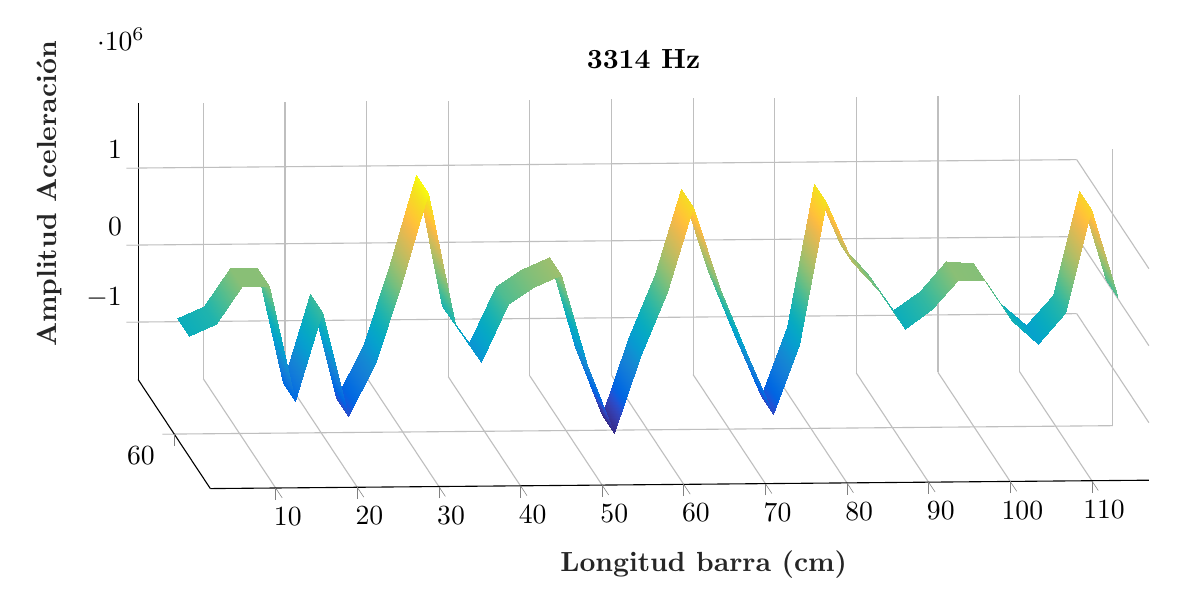
\begin{tikzpicture}

\begin{axis}[%
width=12.837cm,
height=5cm,
at={(0cm,0cm)},
scale only axis,
xmin=2,
xmax=117,
tick align=outside,
xlabel style={font=\bfseries\color{white!15!black}},
xlabel={Longitud barra (cm)},
ymin=45,
ymax=75,
zmin=-1746624.83590174,
zmax=1840864.28413928,
zlabel style={font=\bfseries\color{white!15!black}},
zlabel={Amplitud Aceleración},
view={-4.4}{21.6},
axis background/.style={fill=white},
title style={font=\bfseries},
title={3314 Hz},
axis x line*=bottom,
axis y line*=left,
axis z line*=left,
xmajorgrids,
xminorgrids,
ymajorgrids,
yminorgrids,
zmajorgrids,
zminorgrids
]

\addplot3[%
surf,
shader=interp, colormap={mymap}{[1pt] rgb(0pt)=(0.2081,0.1663,0.5292); rgb(1pt)=(0.211624,0.189781,0.577676); rgb(2pt)=(0.212252,0.213771,0.626971); rgb(3pt)=(0.2081,0.2386,0.677086); rgb(4pt)=(0.195905,0.264457,0.7279); rgb(5pt)=(0.170729,0.291938,0.779248); rgb(6pt)=(0.125271,0.324243,0.830271); rgb(7pt)=(0.0591333,0.359833,0.868333); rgb(8pt)=(0.0116952,0.38751,0.881957); rgb(9pt)=(0.00595714,0.408614,0.882843); rgb(10pt)=(0.0165143,0.4266,0.878633); rgb(11pt)=(0.0328524,0.443043,0.871957); rgb(12pt)=(0.0498143,0.458571,0.864057); rgb(13pt)=(0.0629333,0.47369,0.855438); rgb(14pt)=(0.0722667,0.488667,0.8467); rgb(15pt)=(0.0779429,0.503986,0.838371); rgb(16pt)=(0.0793476,0.520024,0.831181); rgb(17pt)=(0.0749429,0.537543,0.826271); rgb(18pt)=(0.0640571,0.556986,0.823957); rgb(19pt)=(0.0487714,0.577224,0.822829); rgb(20pt)=(0.0343429,0.596581,0.819852); rgb(21pt)=(0.0265,0.6137,0.8135); rgb(22pt)=(0.0238905,0.628662,0.803762); rgb(23pt)=(0.0230905,0.641786,0.791267); rgb(24pt)=(0.0227714,0.653486,0.776757); rgb(25pt)=(0.0266619,0.664195,0.760719); rgb(26pt)=(0.0383714,0.674271,0.743552); rgb(27pt)=(0.0589714,0.683757,0.725386); rgb(28pt)=(0.0843,0.692833,0.706167); rgb(29pt)=(0.113295,0.7015,0.685857); rgb(30pt)=(0.145271,0.709757,0.664629); rgb(31pt)=(0.180133,0.717657,0.642433); rgb(32pt)=(0.217829,0.725043,0.619262); rgb(33pt)=(0.258643,0.731714,0.595429); rgb(34pt)=(0.302171,0.737605,0.571186); rgb(35pt)=(0.348167,0.742433,0.547267); rgb(36pt)=(0.395257,0.7459,0.524443); rgb(37pt)=(0.44201,0.748081,0.503314); rgb(38pt)=(0.487124,0.749062,0.483976); rgb(39pt)=(0.530029,0.749114,0.466114); rgb(40pt)=(0.570857,0.748519,0.44939); rgb(41pt)=(0.609852,0.747314,0.433686); rgb(42pt)=(0.6473,0.7456,0.4188); rgb(43pt)=(0.683419,0.743476,0.404433); rgb(44pt)=(0.71841,0.741133,0.390476); rgb(45pt)=(0.752486,0.7384,0.376814); rgb(46pt)=(0.785843,0.735567,0.363271); rgb(47pt)=(0.818505,0.732733,0.34979); rgb(48pt)=(0.850657,0.7299,0.336029); rgb(49pt)=(0.882433,0.727433,0.3217); rgb(50pt)=(0.913933,0.725786,0.306276); rgb(51pt)=(0.944957,0.726114,0.288643); rgb(52pt)=(0.973895,0.731395,0.266648); rgb(53pt)=(0.993771,0.745457,0.240348); rgb(54pt)=(0.999043,0.765314,0.216414); rgb(55pt)=(0.995533,0.786057,0.196652); rgb(56pt)=(0.988,0.8066,0.179367); rgb(57pt)=(0.978857,0.827143,0.163314); rgb(58pt)=(0.9697,0.848138,0.147452); rgb(59pt)=(0.962586,0.870514,0.1309); rgb(60pt)=(0.958871,0.8949,0.113243); rgb(61pt)=(0.959824,0.921833,0.0948381); rgb(62pt)=(0.9661,0.951443,0.0755333); rgb(63pt)=(0.9763,0.9831,0.0538)}, mesh/rows=36]
table[row sep=crcr, point meta=\thisrow{c}] {%
%
x	y	z	c\\
3.25	58	-377706.369151453	-377706.369151453\\
3.25	63	-377706.369151453	-377706.369151453\\
6.5	58	-230431.381425917	-230431.381425917\\
6.5	63	-230431.381425917	-230431.381425917\\
9.75	58	258349.215869406	258349.215869406\\
9.75	63	258349.215869406	258349.215869406\\
13	58	262718.854373274	262718.854373274\\
13	63	262718.854373274	262718.854373274\\
16.25	58	-1238047.75100296	-1238047.75100296\\
16.25	63	-1238047.75100296	-1238047.75100296\\
19.5	58	-87882.5621233947	-87882.5621233947\\
19.5	63	-87882.5621233947	-87882.5621233947\\
22.75	58	-1434433.86481331	-1434433.86481331\\
22.75	63	-1434433.86481331	-1434433.86481331\\
26	58	-770785.637285279	-770785.637285279\\
26	63	-770785.637285279	-770785.637285279\\
29.25	58	257013.808469518	257013.808469518\\
29.25	63	257013.808469518	257013.808469518\\
32.5	58	1447897.99761056	1447897.99761056\\
32.5	63	1447897.99761056	1447897.99761056\\
35.75	58	-253344.951826411	-253344.951826411\\
35.75	63	-253344.951826411	-253344.951826411\\
39	58	-745665.726331658	-745665.726331658\\
39	63	-745665.726331658	-745665.726331658\\
42.25	58	2436.90522679345	2436.90522679345\\
42.25	63	2436.90522679345	2436.90522679345\\
45.5	58	210611.069676038	210611.069676038\\
45.5	63	210611.069676038	210611.069676038\\
48.75	58	363093.687032838	363093.687032838\\
48.75	63	363093.687032838	363093.687032838\\
52	58	-802070.859501838	-802070.859501838\\
52	63	-802070.859501838	-802070.859501838\\
55.25	58	-1694271.47583777	-1694271.47583777\\
55.25	63	-1694271.47583777	-1694271.47583777\\
58.5	58	-708672.837375235	-708672.837375235\\
58.5	63	-708672.837375235	-708672.837375235\\
61.75	58	137376.729444642	137376.729444642\\
61.75	63	137376.729444642	137376.729444642\\
65	58	1234281.46585062	1234281.46585062\\
65	63	1234281.46585062	1234281.46585062\\
68.25	58	168819.043376029	168819.043376029\\
68.25	63	168819.043376029	168819.043376029\\
71.5	58	-652534.146281432	-652534.146281432\\
71.5	63	-652534.146281432	-652534.146281432\\
74.75	58	-1457959.12897457	-1457959.12897457\\
74.75	63	-1457959.12897457	-1457959.12897457\\
78	58	-571946.842412846	-571946.842412846\\
78	63	-571946.842412846	-571946.842412846\\
81.25	58	1282474.6072148	1282474.6072148\\
81.25	63	1282474.6072148	1282474.6072148\\
84.5	58	507023.26100252	507023.26100252\\
84.5	63	507023.26100252	507023.26100252\\
87.75	58	118565.742381999	118565.742381999\\
87.75	63	118565.742381999	118565.742381999\\
91	58	-366008.703157271	-366008.703157271\\
91	63	-366008.703157271	-366008.703157271\\
94.25	58	-116758.240902097	-116758.240902097\\
94.25	63	-116758.240902097	-116758.240902097\\
97.5	58	263920.433730999	263920.433730999\\
97.5	63	263920.433730999	263920.433730999\\
100.75	58	240119.798961667	240119.798961667\\
100.75	63	240119.798961667	240119.798961667\\
104	58	-286810.23527537	-286810.23527537\\
104	63	-286810.23527537	-286810.23527537\\
107.25	58	-578084.353191073	-578084.353191073\\
107.25	63	-578084.353191073	-578084.353191073\\
110.5	58	-179084.129442558	-179084.129442558\\
110.5	63	-179084.129442558	-179084.129442558\\
113.75	58	1162466.28463221	1162466.28463221\\
113.75	63	1162466.28463221	1162466.28463221\\
117	58	0	0\\
117	63	0	0\\
};
\end{axis}
\end{tikzpicture}% }
		\caption{Amplitud de la aceleración en el modo número 8.}
\end{figure}
\FloatBarrier

\section{Ejemplo avanzado}

El potencial del paquete \textit{Tikz} es muy alto, se pueden realizar muchísimas cosas. En la red se facilitan muchos ejemplos para poder ver el funcionamiento y aprender. Existen hilos donde la gente publica sus mejores diseños de \textit{Tikz} como en \url{https://tex.stackexchange.com/questions/158668/nice-scientific-pictures-show-off} o páginas donde facilitan muchas plantillas como \url{http://www.texample.net/tikz/examples/all/}.
\par Un ejemplo de lo que se puede llegar a conseguir es el siguiente:
% Vector Styles
\tikzset{
  load/.style   = {ultra thick,-latex},
  stress/.style = {-latex},
  dim/.style    = {latex-latex},
  axis/.style   = {-latex,black!55},
}

% Drawing View
\tikzset{dimetric2/.style={
  x={(0.935cm,-0.118cm)},
  y={(0.354cm, 0.312cm)},
  z={(0.000cm, 0.943cm)},
}}
\begin{figure}[ht]
\centering
  \begin{tikzpicture}
    \node (origin) at (0,0) {}; % shift relative baseline
    \coordinate (O) at (2,3);
    \draw[fill=gray!10] (O) circle (1);
    \draw[fill=white] (O) circle (0.75) node[below,yshift=-1.125cm] {Corte trasversal};
    \draw[dim] (O) ++(-0.75,0) -- ++(1.5,0) node[midway,above] {$d_i$};
    \draw[dim] (O) ++(-1,1.25) -- ++(2,0) node[midway,above] {$d_o$}; 
    \foreach \x in {-1,1} {
      \draw (O) ++(\x,0.25) -- ++(0,1.25);
    }
  \end{tikzpicture}
  \begin{tikzpicture}[dimetric2]
        \coordinate (O) at (0,0,0);
        \draw[axis] (O) -- ++(6,0,0) node[right] {$x$};
        \draw[axis] (O) -- ++(0,6,0) node[above right] {$y$};
        \draw[axis] (O) -- ++(0,0,6) node[above] {$z$};
        \draw[fill=gray!50] (0,0,-0.5) circle (0.5); 
        \fill[fill=gray!50] (-0.46,-0.2,-0.5) -- (0.46,0.2,-0.5) -- (0.46,0.2,0) -- (-0.46,-0.2,0) -- cycle;
        \draw[fill=gray!20] (O) circle (0.5);
    \draw (0.46,0.2,-0.5) -- ++(0,0,0.5) node[below right,pos=0.0] {Soporte fijo};
    \draw (-0.46,-0.2,-0.5) -- ++(0,0,0.5);
    \draw[fill=gray!10] (O) circle (0.2);
    \fill[fill=gray!10] (-0.175,-0.1,0) -- (0.175,0.1,0) -- ++(0,0,4) -- (-0.175,-0.1,4) -- cycle;
    \draw (-0.175,-0.1,0) -- ++(0,0,4);
    \draw (0.175,0.1,0) -- ++(0,0,4) node[right,midway] {Poste de acero};
    \draw (4,0,3.95) -- ++(0,0,-1);
    \foreach \z in {0.5,0.75,...,5} {
      \draw[-latex] (-2*\z/5-0.2,0,\z) -- (-0.2,0,\z);
    }
    \draw[load] (0,0,4) -- ++(0,0,-1.25) node[right,xshift=0.1cm] {$F_{z1}$};
    \draw[fill=gray!20] (-0.25,-0.25,5) -- (4,-0.25,5) -- (4,+0.25,5) -- (-0.25,+0.25,5) -- cycle; 
    \draw[fill=gray!50] (+4.00,-0.25,4) -- (4,+0.25,4) -- (4,+0.25,5) -- (+4.00,-0.25,5) -- cycle; 
    \draw[fill=gray!10] (-0.25,-0.25,4) -- (4,-0.25,4) -- (4,-0.25,5) -- (-0.25,-0.25,5) -- cycle; 
    \draw (4.05,0,4) -- ++(1,0,0);
    \draw (4.05,0,5) -- ++(1,0,0);
    \draw[dim] (4.5,0,0) -- ++(0,0,4) node[midway,right] {$h_1$};
    \draw[dim] (4.5,0,4) -- ++(0,0,1) node[midway,right] {$h_2$};
    \draw[dim] (0,0,3.4) -- ++(4,0,0) node[midway,below] {$b_2$};
    \coordinate (P) at (2,-0.25,4.5);
    \draw (P) -- ++(0,0,0.25);
    \draw (P) -- ++(0.25,0,0);
    \draw[dim] (2.125,-0.25,4.5) -- ++(0,0,-0.5) node[midway,right] {$z_1$};
    \draw[dim] (2,-0.25,4.625) -- ++(-2,0,0) node[midway,below] {$x_1$};
    \draw[load] (2,-2.45,4.5) -- ++(0,2.2,0) node[pos=0.0,right,xshift=0.08cm] {$F_{y1}$};
    \draw[axis,dashed,-] (O) -- (0,0,5);
    \draw (0,0,5.5) -- ++(4,0,0) node[midway,above] {$w_{z}$};
    \foreach \x in {0,0.25,...,4} {
      \draw[-latex] (\x,0,5.5) -- ++(0,0,-0.5);
    }
    \draw (-0.2,0,0) -- ++(-2,0,5) node[above,xshift=0.5cm] {$w_{x}=\frac{z}{h_1+h_2} w_0$};
  \end{tikzpicture}
\caption{Señal realizada con Tikz, sin imágenes.}
\label{senyal}
\end{figure}
\FloatBarrier
